\documentclass{article}
\usepackage{amssymb, amsmath}
\usepackage{anysize}
\usepackage{graphicx}
\marginsize{2cm}{2cm}{2cm}{2cm}
\newcommand{\bs}[1]{\boldsymbol{#1}}
\begin{document}
Started 10/3 2013 or somewhere around there.


\textbf{HughesLiuZimmermann1981}
\begin{itemize}
\item Material domain in motion??.
\item Try to understand examples better.
\end{itemize}

\textbf{BraessWriggers2000}
\begin{itemize}
\item Free surface flow as an example of the ALE method permitting a good mesh (no distortion) and an accurate description of boundaries at the same time (due to Eulerian description being used horizontally and Lagrangian description vertically).
\item I should emphasize that the convective velocity isn't physical!
\item Aspect ratio of elements as r\_out/r\_in.
\item (p.103) In case of Lagrangian description: mesh distortion a problem, but can be solved using remeshing. Computationally costly though, and a source of discretization errors.
\item Remeshing is used.
\end{itemize}

\textbf{FrancaFarhat1995}
\begin{itemize}
\item Stabilization operator
\[P(v) = -\sigma v + a\nabla v + \kappa\Delta v\]
instead of
\[P(v) = \sigma v + a\nabla v + \kappa\Delta v\]
\end{itemize}

\textbf{BankWelfert1990}
\begin{itemize}
\item 
\end{itemize}

\textbf{Stromberg2011}
\begin{itemize}
\item Uses decoupled thermomechanical equations.
\item Doesn't seem to model heat exchange with environment.
\item Coded in Fortran? Not clear.
\item Global sliding assumed!
\item S-U-stabilization implemented.
\item Why call the kinematical model "Eulerian"? Due to no translation of wheel? (Then, no linear acceleration effects?)
\item No problems with energy dissipation?
\item Only wheel--brake block contact. No translation.
\end{itemize}

\textbf{PaukYevtushenko1997}
\begin{itemize}
\item Sliding using an Eulerian approach.
\item The effect of rail chill shown (more prominent for higher Pe).
\end{itemize}

\textbf{WauerSchweizer2010}
\begin{itemize}
\item Many good thermoelasticity-references in the beginning.
\item Eulerian disc-brakeblock-model (as in Stromberg2011) \emph{using cylindrical coordinates}.
\item No mention of numerical instability or measures to mitigate it, probably because there is none, due to the use of cyl. coords.
\item Insight: If \emph{any} convection, then not Lagrangian description. If \emph{any} movement of nodes, then not Eulerian description. Therefore ALE.
\end{itemize}

\textbf{SchweizerWauer2001}
\begin{itemize}
\item Very nice introduction, discussing thermomechanical coupling.
\item Metals -- polychrystalline. Rubber -- polymeric.
\end{itemize}

\textbf{Galantucci1999}
\begin{itemize}
\item Lagrangian formulation of hot rolling ($>$800 deg used). Rolling 2$\pi$/4 and 2$\pi$.
\end{itemize}

\textbf{Belytschko1980}
\begin{itemize}
\item FSI application with ALE (called quasi-Eulerian here).
\end{itemize}

\textbf{Hughes1995}
\begin{itemize}
\item Stabilized methods originate from a particular class of subgrid scale methods.
\item $\tau$ can be defined exactly: it can be derived from first principles.
\item Check Hughes publications following this paper.
\item Bubbles identified as approximations of element Green's functions.
\item Bubbles in the subgrid + static condensation $\approx$ subgrid scale model + assumption of subgrid contribution vanishing on element boundaries.
\item Expression for $\tau$ derived, involves $g(x,y)$.
\end{itemize}

\textbf{AmsdenHirt1973book}
\begin{itemize}
\item Mostly describes the code YAQUI (which uses finite differences).
\item Other techniques L/E/ALE mentioned, e.g. ICE (?).
\item I should check out reference 2 (HirtAmsdenCook1997), it describes the ALE technique in detail.
\end{itemize}

\textbf{HirtAmsdenCook1997}
\begin{itemize}
\item A very simple ALE description seems to be used. It seems to be described in terms of moving mesh points rather than some formulation preceding discretization based on continuum mechanics.
\item Each time step involves 3 phases, the last of which is optional re-zoning: moving vertices to keep a good mesh quality and thereby causing convection. An upwind averaging scheme is here used to avoid numerical instability (p. 209).
\item The method seems so closely tied to the mesh and the practical computational algorithm. They don't start from first principles (continuum mechanics) as for instance Donea \& Huerta, Nackenhorst etc.
\end{itemize}

\textbf{FrancaFarhat1994}
\begin{itemize}
\item In a pure diffusion prolem, the node values at the nodes included in the linear mesh are the same whether linear or quadratic interpolation is used.
\item I'm wondering what the 1D example has to do with bubbles. It seems that linear--quadratic is what's compared, rather than bubbles on/off.
\item But int he 2D example, they use an approximation consisting of a linear interpolation + a higher order bubble (for which they need to introduce an extra node).
\end{itemize}

\textbf{FrancaFrey1992}
\begin{itemize}
\item Compares a stabilization method by Douglas--Wang with the GLS method for Stokes flow.
\item Hints that the pure least-squares method gives too dissipative results for the advection--diffusion equation.
\item Example: 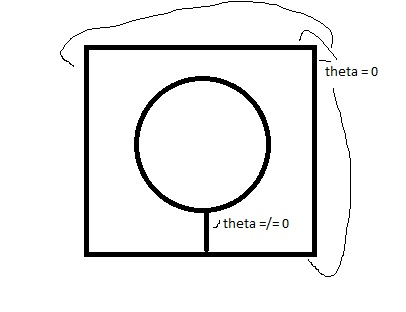
\includegraphics[width=5cm]{figures/FrancaFrey1992_img1.jpg}
\item Example: 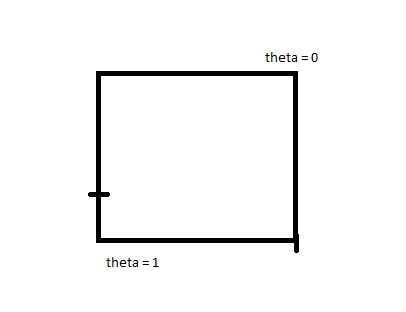
\includegraphics[width=5cm]{figures/FrancaFrey1992_img2.jpg}\\
Here, quad is considerably better than lin for equal number of dofs.
\item Some development in the choice of $\tau$.
\end{itemize}

\textbf{BurmanHansbo2004}
\begin{itemize}
\item Term added to the weak form penalizing gradient jumps across element boundaries.
\item It is said that the source of the added stability is the fact that the edge of operator controls the projection error of the term $\bs{\beta}\cdot\nabla v$ $(\bs{a}\cdot\nabla\theta)$ in the case of convection--diffusion.
\item Some error estimates are given and proven.
\item Something called "shock capturing" is mentioned, which was used in a previous paper. The numerical examples both do and don't use shock capturing.
\end{itemize}

\textbf{GaoHuang2006}
\begin{itemize}
\item Insightful introduction about:
\begin{itemize}
\item Disc brakes, pros and failure modes, including thermomechanical effects.
\item How fatigue cracks initiate and spread.
\item Comment on the assumption of a constant sliding velocity in braking simulations.
\end{itemize}
\item Disc braking model with variable speed (down to 0).
\item The model used uses simplifying geometrical and thermal assumptions that make it very specific to the given application.
\item FEM using ANSYS.
\item On hot spots and how their related temperature spikes can be avoided.
\item Results show fluctuating temperatures and stresses. Up due to frictional heat generation and down due to dissipation/convection. (I don't really understand) when studied point is outside of the contact region (the part in parenthesis above was strikethrough:ed, I don't know what I meant by that). One cycle per revolution.
\item Unclear whether Eulerian or Lagrangian description.
\item Contact model unclear.
\end{itemize}


\textbf{HuertaLiu1988}
\begin{itemize}
\item History of ALE (just as in DoneaHuerta2003book).
\item Spurious oscillations when Galerkin method is used for convection--dominated problems is because the FE equations are not self-adjoint.
\item "The [ALE] reference frame is fixed, but its movement [...] is arbitrary...". If this isn't a contradiction, then what does "fixed" mean in this context?
\item Tsunami, dam-break and sloshing problem considered. Large free-surface motion.
\item The use "a SUPG method for the mesh updating equation". What does this mean?
\item Kinematical description different for each problem, but in general Eulerian in the horizontal direction and Lagrangian in the vertical direction.
\end{itemize}


\textbf{Baiocchi1993}
\begin{itemize}
\item Intro mentions bubbles + static condensation (SC) viewed as the addition of a stabilizing term to the FE problem.
\item Addition of bubbles + SC formulated in abstract form. The resulting stabilization term added to the RHS is derived for the general case...
\item ...and then for two specific examples, one of which is the advection--diffusion problem.
\item If bubble functions + SC is equivalent to the SUPG among others, why does it work better in the rotating disc case? Because the space used for the bubble functions is of a particularly high quality?
\item Paper establishes "a rather general link between two major families of stabilizing techniques". For the first time I guess? Nice.
\end{itemize}

\textbf{BrezziBristeau1992}
\begin{itemize}
\item Similar to Baiocchi1993 (Brezzi \& Franca authors on both). The equivalence between Galerkin + bubbles and stabilized FE methods is established. The limit $\kappa \rightarrow 0$ is investigated.
\item The stability of different methods are investigated quantitatively.
\item Relationship between bubbles and SUPG was first noted in Rogé's thesis (so, I should cite that if I write about it).
\end{itemize}

\textbf{XuJiang2001}
\begin{itemize}
\item Introduction:
\begin{itemize}
\item On rolling contact, where it happens and associated problems (damage phenomena).
\item Stress analysis, of its importance to understand fatigue/wear and how it's done: semianalyt or FEM. \emph{many} references on each method. I should check them out to understand: a) why "semi-"? b) How to do rolling contact with FEM without ALE?
\item Claims to be first paper to do elastic-plastic stress analysis with stick/slip.
\item History of stick/slip, experimental/theoretical.
\item Partial slip more damaging than full?
\end{itemize}
\item This paper: Stresses/deformations due to stick/slip rolling. \underline{Uses analytical load on meshed rail (2D plane strain)}.
\item Uses finite elements!
\item ABAQUS used
\item 2-4 hours per rolling cycle!
\item Results similar to those of JiangSehitoglu1999's semi-analytical theory (next reference in this list)
\end{itemize}

\textbf{JiangSehitoglu1999}
\begin{itemize}
\item Introduction:
\begin{itemize}
\item Distinguishes between engineering/research models for life prediction of rolling contact (references Tallian).
\item Problems with FE models: computationally expensive, convergence issues.
\item Current paper uses a semi-analytical model, shown to agree with FE results.
\end{itemize}
\item Talks about critical plane approaches to fatigue.
\item Stress distribution obtained from Hertzian contact theory. Full slip assumed.
\item Contact pressure distribution assumed to be unaffected by stick/slip, geometry changes, etc.
\end{itemize}

\textbf{Special section}
Summary of my quick look at references 3--13 and 14--24 in \textbf{XuJiang2001} (these groups of references refer to semi-analytical vs. FE-based analysis of rolling contact)

\noindent
\underline{3--13}
\begin{itemize}
\item Semi-analytical: Hertzian contact theory gives stress distribution/deformation in contacting bodies. Numerical methods modelling e.g. inelastic material response or wear or fatigue are used in conjunction with these solutions.
\item Significant gain in computational cost compared to FE methods (see eg. number 9). No convergence problems, especially in 3D.
\item Isn't no. 11 a FE method?
\end{itemize}
\underline{14--24}
\begin{itemize}
\item Papers using elliptic pressure distribution on meshed rail: all of them.
\end{itemize}


\textbf{Kulkarni1991}
\begin{itemize}
\item Introduction:
\begin{itemize}
\item Important to account for thermal effects.
\item Present paper: Transiently elasto-plastic, thermomechanical FE model of 2D frictional rolling contact (of type: analytical Hertz pressure distr. on FE mesh).
\end{itemize}
\item Lets a purely thermal load pass before the thermomechanical one. Why?
\item Fig 9 is nice. Looks just like you'd expect.
\item Observes residual tensile stresses in the rail (an explanation is given).
\end{itemize}

\textbf{Special remark}
Now, let's look at papers on rolling contact including \underline{two} bodies, preferably with AND without ALE. (How is two-body contact without ALE done?)

\textbf{Ibrahimbegovic2003}
\begin{itemize}
\item In short: non-linear dynamics of flexible systems with constraints (large deformations)
\item Rolling contact example exemplifying non-holonomic constraints. But very simple: rigid bodies, no slip.
\item Lagrangian kinematics all the way, it seems.
\end{itemize}

\textbf{Amirouche1993}
\begin{itemize}
\item About dynamic analysis of rolling contact in flexible multibody systems. Large deformations.
\item Intro mentions other rolling contact references and seems to hint at ALE implementations.
\item Node--node contact model used.
\item Eqs. of motion "presented in matrix form making use of Kane's equations and FEM". Chapter 2 contains a derivation. I don't understand a thing.
\item According to Lesser1992, Kane's eqs. are "equations of motion for systems of constrained particles and rigid bodies". So how does it apply to deformable bodies?
\item \textbf{\underline{Very}} coarse mesh used in the wheel--rail rolling contact numerical example.
\end{itemize}

\textbf{Arnold1984}
\begin{itemize}
\item Proof that the MINI element (linear shape functions + bubble function) satisfies the inf-sup condition for the Stokes problem (coupled velocity-pressure).
\end{itemize}

\textbf{BrezziMarini1998}
\begin{itemize}
\item Residual-free bubbles were "recently introduced" in 1997.
\item Great description of "layers" (boundary and internal) in which the solution changes abruptly due to convection dominated flow. Also on how a Galerkin approach with a mesh that is too coarse to resolve these layers leads to numerical oscillations spreading all over the domain. WHY?? (see DoneaHuerta2003book?)
\item On the relation between SUPG and bubble functions: the problem of choosing $\tau$ can be transferred to the problem of choosing a suitable bubble space, since $\tau$ can be expressed exactly as soon as the latter has been done.
\item[Q] If SUPG and bubble function method are equivalent, why do bubbles (but not SUPG) work in my case (especially since I choose the extra node $P$ in a fairly ad hoc way)? Hmm, bubbles \emph{do} work better than SUPG in this paper, see next Q.
\item Paper is dedicated to approximationg $b_k$, the function involved in the exact expression for $\tau$.
\item Strategy: Look for an approximation to $b_k$ in the shape of a pyramid (i.e. look for a solution to the differential equation (35), which governs $b_k$, in the shape of a pyramid). Unknowns: position of $P$ and height of pyramid.
\item Method used: Choose $P$ along the thin line in the triangles in the figure (the thin line can be chosen parallel to the convective velocity field as well). Note that in the left figure, there is one outflow edge, while in the other there is two. The thin line goes from either the corner opposite the only outflow edge or from the corner in between the two outflow edges, and to the middle of the opposite side.
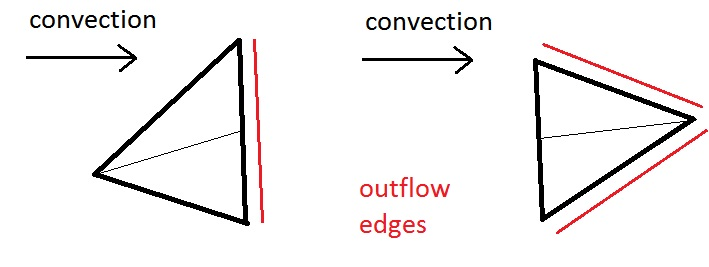
\includegraphics[width=5cm]{figures/BrezziMarini1998_img1.jpg}
\item[Q] Examples show how SUPG is over-diffusive compared to bubbles and refined Galerkin. But I wonder how coarse Galerkin would look. Over-diffusive (damped) or just oscillatory?
\item They don't seem to mention how $\tau$ is chosen in the SUPG method they use in the examples. Is there a standard choice?
\item[Q] Can it be that the pure over-diffusion that happens in my case (i.e. no oscillation) is due to the absence of boundary layers (since the convection streamlines are all closed: \underline{no outflow boundary}).
\item One more thing: this paper doesn't assume that convection dominates (in that case, finding a suitable bubble space is allegedly easy), but offers a method for the general case.
\end{itemize}

\textbf{BrezziHauke2003}
\begin{itemize}
\item Introduction:
\begin{itemize}
\item First paper on RFB (one I can't get) is Brezzi, Russo: "Choosing bubbles for advection--diffusion problems".
\item[Q] Should I talk about "advection" rather than "convection"?
\item Their point was to find a suitable value for $\tau$.
\item Stabilization (or removing the need for it, rather) by proper choice of grid!
\item Current paper merges the above and bubbles.
\end{itemize}
\item RFB: The bubble space is $H_0^1(K)$, i.e. all functions with a continuous first derivative, with the element $K$ as support and zero at $\partial K$.
\item Origin of the name Residual Free!!!
\item Elaborated: In the RFB approach, the approximation is enriched by a bubble function in each element, taken from the space $H_0^1(K)$. This enriched basis function ($V_L + V_B$) is capable of exactly satisfying the governing equation (the strong form) in each element ($\mathcal{L}u = f$, say), hence "Residual free".
\item Interesting observation that if bubbles are the same type of function as the approximation (e.g. p.w. linear), then the process of adding extra nodes locally in each element and condensing is really just the same thing as "smart" mesh refinement (since condensation -- being optional -- doesn't change the mathematical nature of the procedure).
\item[Q] Maybe I don't get good effects using bubbles in the rail because the nodes there are incorrectly placed? How would the exact bubbles look? In the figure below. a) shows how I do it in Paper 2--4: placement of the extra node (red dot) along a line that is parallel with the convection stream line, and that intersects the centroid (black dot) of the triangle. b) How I perhaps should place it instead, which is based on c) which I guess is some kind of solution to the convective heat equation across the triangle.
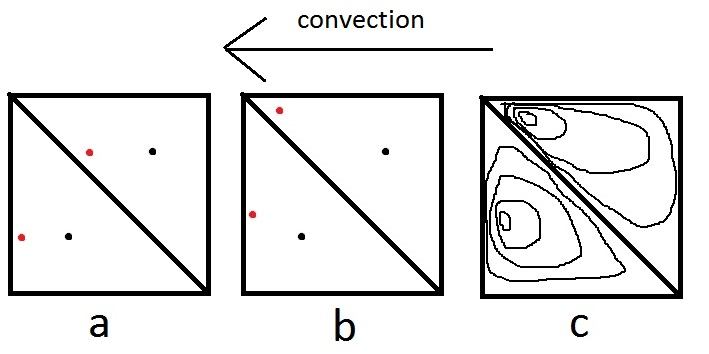
\includegraphics[width=5cm]{figures/BrezziHauke2003_img1.jpg}
\end{itemize}

\textbf{MouradDolbow2007}
\begin{itemize}
\item Not particularly relevant. Also, I don't really understand what is meant by "embedded interfaces".
\item They admit that their choice of bubble space is naive. I identified with that.
\end{itemize}

\textbf{Zeid1981}
\begin{itemize}
\item Quite sophisticated FEM-based contact formulation from a LONG time ago: friction, rigid rail, "Galilean" ($\Leftrightarrow$ Eulerian I guess) transform, unsure of if the contact formulation is more like PM or LMM, purely mechanical case.
\item I don't understand what the Galilean transform does.
\end{itemize}

\textbf{Padovan1987}
\begin{itemize}
\item Part 1/3 of this series of papers.
\item Very sophisticated wheel--rail contact model: 3D, simulation of bumps/holes, viscoelasticity + all of what was in Zeid1981. Still only mechanical though.
\item[R] Search for keywords "thermomechanical rolling contact" in the next search for papers.
\item Coriolis acc. included in formulation. Do I have it in mine? Probably, but which term is it?
\item This paper contains field equations, material model and FEM formulation.
\end{itemize}

\textbf{Kennedy1987}
\begin{itemize}
\item Part 2/3 of this series of papers.
\item Contains 3D formulation, shell formulation, contact formulation (in 3D), and numerical examples.
\item Purely mechanical, so high speeds not surprising. Rigid ground when included.
\item Same Galilean transform here as in Zeid1981?
\item Pantographing mentioned: it is the antenna-like assembly of thin metal "sticks" that connects e.g. trams to the power lines above them.
\end{itemize}

\textbf{Nakajima1987}
\begin{itemize}
\item Part 3/3 of this series of papers.
\item When they talk about "slip--stick" situation is these papers, do they mean total slip/total stick or mixed, as in the examples in my last two papers?
\item[R] Having a rigid rail would enable me to implement a non-smooth contact surface that wouldn't be as "cheating" as the one in paper 1 for instance.
\item Contains contact impact methodology and numerical examples, involving rolling over bumps (triangular protrusions) and holes (triangular depressions)
\end{itemize}

\textbf{ZavariseWriggers1992\_2}
\begin{itemize}
\item Introduction:
\begin{itemize}
\item Constant penalty parameters (for \underline{mechanical/thermal} contact) not enough to accurately model contact behaviour.
\item Micro-geometry important to take into account, especially (?) for macroscopically smooth surfaces. Current paper will do this.
\item Clean surfaces, no friction assumed (no rolling contact of course).
\end{itemize}
\item Thermal contact resistance is modelled as three resistors in parallel: these correspond to thermal resistances due to spots, gas and radiation.
\item Relations for $c_i = 1/R_i$ for spots and gas derived. They depend on microgeometrical considerations such as real contact area (dependent on $p$), cavity size (dependent on $p$) and statistical parameters.
\item Comparison with experiments gives unknown parameters. They note: this is no ordinary curve fitting that only gives a model applicable to a narrow set of situations, but a calibration of a sophisticated theoretical model.
\item FEM residuals are consistently linearized so that Newton's method can be used.
\item Model is concluded to give high precision and a detailed understanding of mechanisms in the contact zone.
\item No elaboration on mechanical contact formulation, \underline{they probably just use a constant penalty parameter}, as in ZavariseWriggers1992.
\end{itemize}

\textbf{ZavariseWriggers1992}
\begin{itemize}
\item Introduction:
\begin{itemize}
\item They make a point about how primitive the constant contact conductivity models are in comparison with theirs.
\item Another paper about roughly the same thing as in ZavariseWriggers1992\_2: Development of a thermomechanical contact element based on material laws representing "true" contact mechanisms.
\end{itemize}
\item Frictionless contact, clean (oxide-free) surfaces assumed (allegedly complicated to treat non-clean surfaces). Frictional formulation under construction (said in conclusions).
\item Uses same 5-node contact element that I do.
\item \underline{Constant normal stiffness used!} They almost apologize for it, see p. 771 "we have focussed [sic] our interest more on the thermomechanical coupling".
\end{itemize}

\textbf{SchreflerZavarise1993}
\begin{itemize}
\item More of the same (microgeometrical thermomechanical contact formulation).
\item Nice passage in the introduction about required accuracy of the contact formulation depending on implementation.
\item Much more detailed/sophisticated mechanical contact formulation here than in the 2 previous papers.
\end{itemize}

\textbf{WriggersZavarise1993\_2}
\begin{itemize}
\item Pure micromechanics here (\underline{no thermal contact}).
\item No friction, small displacements, nodal contact formulation.
\item Augmented Lagrangian technique used.
\end{itemize}

\textbf{WriggersZavarise1993}
\begin{itemize}
\item Node-to-node formulation. No friction.
\item Microscopic statistical interface laws both for mechanical \& thermal problem.
\item Remark 1 on p. 50 discusses element area-dependent normal mechanical penalty parameter.
\item Interfacial thermal conductivity depends on pressure.
\end{itemize}


\textbf{WriggersMiehe1994}

\begin{itemize}
\item The paper presents a microgeometrical contact interface model for thermomechanical frictional contact.
\item Contact geometry described in detail.
\item Sophisticated interface laws for normal contact stress and contact heat flux given. Seems like no mention of frictional heat generation? Slip is split into an elastic part and a plastic part.
\item "The resistance agains heat transfer is mainly due to the low percentage of physical surface area which is really in contact."
\item Thermoelasticity constitutive response assumed.
\item Gough--Joule coupling effect included (no mention about neglecting it).
\item A staggered scheme (problem split into "a purely mechanical subproblem (M) at frozen temperature" (called a "predictor") and "a purely thermal subproblem (T) at frozen configuration (called a "corrector")). The algorithm is said to be identical to the one suggested in Argyris and Doltsinis [16].
\item Numerical examples provided. Most of them feature a thermoelastic body pressed against a rigid but heat-conducting body. Idealized thermal isolation or fixed temperatures are assumed at surfaces.
\end{itemize}

\textbf{Nackenhorst2004}
\begin{itemize}
\item General summary: Lays out the mathematical foundations for elastic, transient rolling contact based on an ALE kinematical description. The kin. descr., balance laws, weak form, rolling contact kinematics are discussed + FE approach of stationary rolling including linearizations.
\item Introduction:
\begin{itemize}
\item ALE-like methods used before (goes back to Padovan, Oden\&Lin). Inelastic material behaviour has even been addressed in the ALE context (engineering approaches relying on structured meshes I think (references [10], [29])) or the Streamline Upwind-based method of LeTallec and Rahier. However, Nackenhorst says, previous works do not handle the contact problem stringently, and don't provide a sound mathematical basis for inelastic or rate dependent material behaviour.
\end{itemize}
\item He uses 3 domains. All use ground-fixed coordinate systems! His no. 1 = my no. 1; his no. 3 = my no. 4; his no. 2 is my no. 2 but with a ground-fixed coord. syst; his no. 3 is my no. 4 but with a ground-fixed coord. syst! I.e. his $\boldsymbol{w}$ (my $\boldsymbol{\bar{v}}$) contains a translational part! Despite the above, his \underline{displacements} are the same as mine.
\item His $\boldsymbol{w}$ is called the "guiding velocity". \emph{His} "convective velocity" is $\mathrm{Grad}\boldsymbol{\phi}\cdot\boldsymbol{w}$ which I'll have to agree is the true convective velocity).
\item[Q] How do we handle mass balance? Just by $\hat{\rho} = \rho J$? Aha, we assume homogeneity.
\item He performs a symmetrization by partial integration (p. 4306).
\item I actually think he forgets a term in eq. (28).
\item He computes the term involving $\boldsymbol{\hat{n}}\cdot\boldsymbol{w}$! For perfectly round boundaries, this term vanishes. I therefore neglect it. Nackenhorst mentions that it is best to include it, however, since it has a real influence in discretized geometries. Neglecting it introduces an error.
\item In discussion of FE formulation, he restricts the discussion to stationary rolling contact and a rigid rolling surface.
\item Unsure of whether he uses a staggered solution procedure or if he just computes successively refined start guesses, like I do (probably the former, based on later papers).
\end{itemize}









\textbf{ZiefleNackenhorst2007}
\begin{itemize}
\item Introduction:
\begin{itemize}
\item So Oden and Lin and Padovan (and Zeid I guess) are the first examples of FEM being used for rolling contact. They used a relative kinematics approach or whatever it's called. (I guess it is impossible to model rolling contact using FEM using a purely Lagrangian description.) ALE is more general though.
\item "[...] the history of particles which initially got into contact has to be traced to evaluate the friction law". Why? Aren't slip velocities enough? "A common procedure [regarding treatment of frictional contact within an ALE context] is the penalization of the slip velocities which are computed directy within the relative kinematic framwork". Is that what I'm doing?. "A further complication arises from the fact that by this approach the tangential contact traction is not computed directly from a constitutive law". I don't understand this, I thought that was what I was doing.
\end{itemize}
\item The slip distances can be computed from the slip velocities by temporal integration, which can be exchanged for spatial integration due to the fact that time derivatives are exchanged for spatial derivatives in the convective description (is this true for the transient case as well?)
\item Slip distances introduced as extra variables.
\item "Once [the slip distribution has been obtained], the standard concepts for the treatment of frictional contact problems can be used, see eg. [18] [a paper by Wriggers].". Why is the slip distance (undifferentiated) needed in a friction law? How is "slip distance = 0" a valid stick condition?
\end{itemize}

\textbf{ZiefleNackenhorst2007\_2}
\begin{itemize}
\item Introduction:
\begin{itemize}
\item "First approaches on the numerical treatment of rolling contact by finite element methods based on rather simple relative kinematic formulations...". Reference given to Oden and Lin.
\item Check out reference 6 (Faria et. al.). I supposed to mention ALE (but I don't find any explicit reference to it, not by that name anyway).
\item Claims that ABAQUS can handle treatment of inelastic material parameters in an ALE-context. I didn't find anything on this though. Perhaps they call it something other than ALE.
\item "No sound mathematical basis for the treatment of inelastic material properties within the ALE-framework is available so far, which for example enables for error estimation based on computed results. This contribution is aimed to close these gaps".
\end{itemize}
\item Insight: I should know the physical interpretation of all my terms.
\item An additional update procedure for the internal variables has to be provided. This requires tracing the material particles as they move through the fixed FE mesh. This problem is well known in fluid mechanics. 
\item Insight from the above: Any advection-related problem of the ALE approach can probably be found (as well as its solution) in fluid mechanics.
\item In the ALE context, time derivatives in the advection equation are replaced by spatial derivatives (at least in the stationary case).
\item Perhaps "convection": the mathematical concept and "advection": specifically referring to the transport of physical quantities.
\item The "advection equation" is solved to update the internal variables.
\item Different numerical schemes and associated stabilization methods are compared. This is said: "The upstream method is stable, but suffers strongly under diffusion effects". I'm wondering if these are the same as those we observe in paper 2. Perhaps not, since this is 1D.
\item Overshoot-effects result from differences between inflow and the outflow within one element.
\item A fractional-step method (a staggered approach) is used to incorporate the solution of the advection equation in the FE-problem: 1. Solve nonlinear ALE rolling contact problem. 2. Smooth out internal variables for a  $C^0$-smooth representation. 3. Solution of the advection problem by TDG-schema.
\item Question regarding part 2 above: Isn't information lost as the internal variable data is smoothed out in coarser regions of the mesh?
\item As material particles are convected through the contact region, the contact pressure distribution becomes asymmetric for medium convective velocities: for high conv. vel.: no relaxation, for low conv. vel.: total relaxation.
\item One disadvantage of the ALE approach is additional computational effort when inelastic material properties have to be taken into account.
\end{itemize}

\textbf{ZiefleNackenhorst2008}
\begin{itemize}
\item Seems like a combination of the last two papers.
\item Introduction:
\begin{itemize}
\item ALE methods have been developed rapidly in other fields of engineering application, i.e. FSI and metal forming processes (see review paper [13]).
\item Traditional engineering approaches to treatment of inelastic material properties involves integrating the history along predefined rings of integration points (e.g. Faria, Oden/Lin). However, this poses a problem with unstructured meshes and isn't built upon a sound mathematical basis. Le Tallec and Rahier [22] represents a first step towards something more mathematically sound.
\end{itemize}
\item Insight: I should include the expression for $\boldsymbol{v}$ as well and discuss terms such as "guiding velocity" and actual convective velocity.
\item "the accurate and efficient numerical solution of advection equations is still part of the current research in the field of computational fluid dynamics". Implying that ALE approaches can benefit from this research as well.
\item "The TDG approach uses a coupled space-time-discretization instead of the common concept of semi-discretization" apparently.
\item The smoothing out of the internal variables is said to be performed using a "super-convergent patch recovery technique".
\item Regarding Figure 7 of the rolling kinematics. Isn't this a very idealized picture? Is it actually used?
\item "The asymmetric of the contact pressure distribution in the mid-frequency range results in a torque which contributes to the rolling resistance."
\item He uses the slip
\[S = \frac{V_T-V_C}{VT}\]
while I use
\[S = 2\frac{V_T-V_C}{VT+V_C}\]
\item "If inelastic material properties are applied to the model, the computation time increases significantly". I'm wondering: How big is the increase in computational effort in the \emph{Lagrangian} case when inelastic material props are applied?
\item "An explicit scheme has been suggested for the computation of rolling contact problems of inelastic bodies, known as \emph{Fractional-Step}-method from other established ALE-applications, because a fully implicit algorithm seems to be not computable for real life problems yet." Because of excessive computational effort, or what? So the use of the fractional-step method is by necessity rather than by choice?
\item "concerning the frictional rolling contact problem a novel and fully implicit approach for the treatment of tractive rolling contact within the ALE framework for steady-state rolling has been presented". What does "implicit" mean? Requiring iterations?
\item Ref [10] seems to be another good summary paper on ALE methods (by Donea et. al.).
\end{itemize}

\textbf{BrinkmeierNackenhorst2009}
\begin{itemize}
\item Paper focuses on "the transient dynamics response with respect to rolling noise prediction". A modal analysis will be used. The transient response due to excitation from different road surface textures will be investigated next.
\item Quite applied, a little bit outside my area of interest.
\end{itemize}

\textbf{Suwannachit2013}
\begin{itemize}
\item Paper is about thermomechanical analysis of stationary rolling tires using the ALE approach. Large deformations are implemented along with a thermoviscoelastic constitutive model including internal dissipation.
\item Introduction:
\begin{itemize}
\item Internal dissipation is well known to be the main source of temperature rise in tires.
\item "The coupled momentum and energy balance equations are solved with an isentropic operator-split scheme".
\item The transport of inelastic variables during rolling is solved using the TDG method as described in ref. [26].
\end{itemize}
\item Constitutive parameters are temperature-dependent.
\item Viscous hysteresis decreases with increasing environmental temperature and even vanishes eventually. This is captured by their model.
\item They don't want to solve the balance eqs. simultaneously, because the tangent operator is "large" and "nonsymmetrical" in that case. They use a staggered (fractional-step) approach. They here choose the isentropic operator-split method over the isothermal method because the former is unconditionally stable.
\item Frictionless contact considered (and frictional heating is as a consequence not considered) "in order to focus on the heat generation caused by inelastic constitutive behaviour".
\item On the TDG approach: "The major advantage of this approach is its control over numerical inaccuracies, like diffusion and oscillation".
\item "although the global representation of balance equations is time-independent for stationary rolling, integration in time is still needed for the evolution of inelastic strains." A staggered computational scheme is used: i) mechanical subproblem. ii) nonlinear heat conduction, iii) transportation of internal variables.
\item The Gough--Joule effect is neglected (both the thermoelastic and the thermoviscoelastic part of it).
\item For a clear observation of the hysteretic heating, the heat transfer with environmental air is neglected. (perhaps I should have motivated my neglection of this effect better as well).
\item Cool simulation: first inflation (statically), then setting the wheel into rotation, then bringing it into contact with the surface. I guess all this is done "statically" and not transiently.
\item Consistent linearization is employed and quadratic convergence rate of both mech. and therm. subproblems are achieved (using Newton-Raphson iterations).
\item "In our numerical studies, the stationary rolling state was obtained within only few revolutions". I don't get this, isn't everything stationary?
\end{itemize}

\end{document}

%\textbf{key}
%\begin{itemize}
%\item Introduction:
%\begin{itemize}
%\item item
%\end{itemize}
%\item item
%\end{itemize}